\documentclass[tikz,border=3mm]{standalone}
\usetikzlibrary{chains, calc,fit}
\usepackage{varwidth}
\begin{document}
%\definecolor{offwhite}{RGB}{255, 255, 243}  
%%\pagecolor{offwhite}
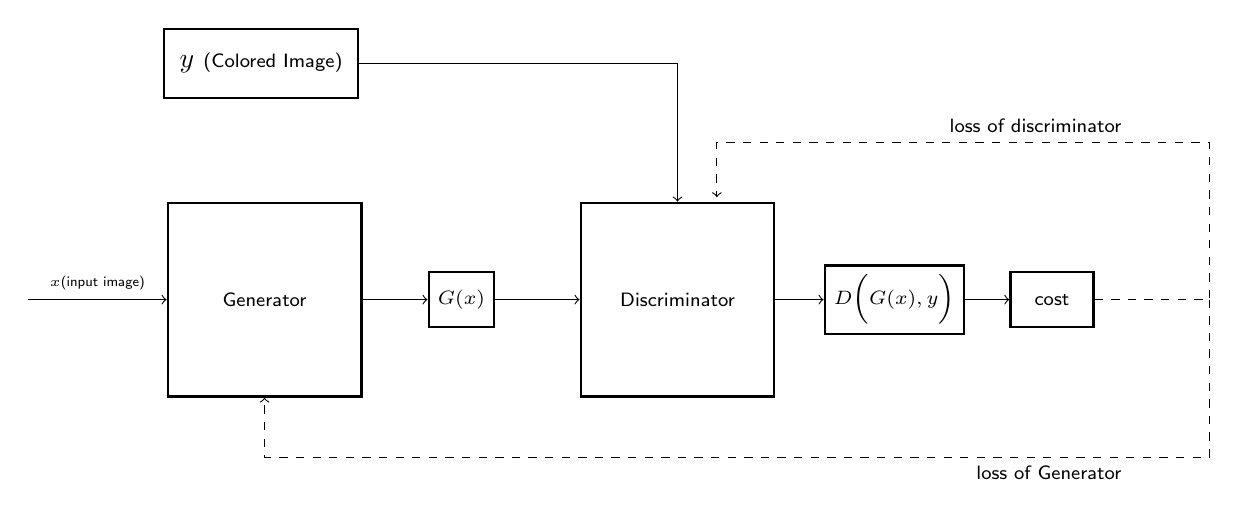
\begin{tikzpicture}[box/.style={draw,thick,minimum width=5em,minimum
    height=10em},arj/.style={semithick,-latex}]
  \begin{scope}[start chain=A going right,oc/.style={join=by arj,on chain},
    font=\sffamily,node distance=1.75em]
   \node(color data)[box,minimum height=2.5em, minimum width=7em,anchor=east]at (1.2,1) {$y$ \scriptsize{(Colored Image)}};
   \node(discriminator)[box,minimum height=7em, minimum width=7em,anchor=west] at (4,-2) {\scriptsize{Discriminator}};
   \draw[->] (color data) -| (discriminator);
   
   \node(generator)[box, minimum height=7em, minimum width=7em] at (0,-2){\scriptsize{Generator}};
   \draw[<-] (generator.west) -- node[above]{\tiny{$x$(input image)}} ++(-5em,0em);
   
   \node(generator func)[box, minimum height = 2em, minimum width = 1em] at (2.5,-2){\scriptsize{$G(x)$}};
   \draw[<-] (generator func) -- (generator);
   \draw[->] (generator func) -- (discriminator);
   
   \node(discriminator func)[box, minimum height = 2em, minimum width = 1em] at (8, -2){\scriptsize{$D\big(G(x),y\big)$}};
   
   \draw[->] (discriminator) -- (discriminator func);
   
   \node(cost)[box, minimum height = 2em, minimum width = 3em] at (10, -2){\scriptsize{cost}};
   
   \draw[->] (discriminator func) -- (cost);
   
   \draw[dashed, ->] (cost) -- (12, -2) -- node[above left=4em]{\scriptsize{loss of discriminator}} (12, 0) -| ($(discriminator) +(0.5,1.3)$);
   
   \draw[dashed, ->] (12,-2) -- node[below left =4em]{\scriptsize{loss of Generator}} (12, -4) -| (generator);
   
  \end{scope}
%   \begin{scope}[shift = {{($(input.south)+(0cm, -2cm)$)}}, start chain=A going right, oc/.style={join=by arj, on chain},
%     font=\sffamily, node distance=1.75em]
%     \node[box,oc]{something};
%   \end{scope}
\end{tikzpicture}
\end{document}